\begin{figure}
  \setlength{\unitlength}{\textwidth}

        \begin{picture}(1,0.74)

      % % % Parkinson Data 
%      \put(0.025,0.5){\includegraphics[width=0.5\unitlength]{../FnP/gnuplot/displacement_amp_collapsed_parkinson.eps}}
%      \put(0.025,0.27){\includegraphics[width=0.5\unitlength]{../FnP/gnuplot/velocity_amp_collapsed_parkinson.eps}}
%      \put(0.495,0.27){\includegraphics[width=0.5\unitlength]{../FnP/gnuplot/velocity_amp_collapsed_re200.eps}}
      
      \put(0.025,0.02){\includegraphics[width=0.5\unitlength]{../FnP/gnuplot/mean_power_collapsed_parkinson.eps}}
      \put(0.495,0.02){\includegraphics[width=0.5\unitlength]{../FnP/gnuplot/mean_power_collapsed_re_200.eps}}
%      \put(0.495,0.5){\includegraphics[width=0.5\unitlength]{../FnP/gnuplot/displacement_amp_collpased_re200.eps}}
      
%      \put(0.23,0.00){ $\displaystyle\frac{c}{\rho\mathcal{A}U}$}
%      \put(0.73,0.00){ $\displaystyle\frac{c}{\rho\mathcal{A}U}$}

      \put(0.28,0.00){\massdamp}
      \put(0.78,0.00){\massdamp}
      
      \put(0.01,0.405){$\displaystyle\frac{V}{D}$}\
       \put(0.01,0.63){$\displaystyle\frac{A}{D}$}
      
      \put(-0.02,0.13){$\displaystyle\frac{P_{m}}{\rho \mathcal{A}U^3 }$}
      
      \put(0.46,0.709){\small(a)}
      \put(0.93,0.709){\small(b)}
      \put(0.46,0.475){\small(c)}
      \put(0.93,0.475){\small(d)}
      \put(0.46,0.225){\small(e)}
      \put(0.935,0.225){\small(f)}
      
    \end{picture}

  \caption{Displacement amplitude, velocity amplitude and mean power as functions of the mass-damping \massdamp. Data presented in (a),(c) and (e)  were calculated using input data at $Re=22300$ obtained by \cite{Parkinson1964} at three different damping ratios: $\zeta=0.0125$ (\ding{83}), $\zeta=0.015$ (\ding{116}) and $\zeta=0.0175$ (\ding{108}). Data presented in (b), (d) and (f)  were obtained using input data at $Re=200$ at three different damping ratios: $\zeta=0.075$ ($\times$), $\zeta=0.1$ (\ding{117}) and $\zeta=0.15$ (+). The collapsed data implies that there is no frequency selection and the tuning parameter of the mechanical side of the system is the damping constant to obtain an optimum power output.}
    \label{fig:collapsed_data}
\end{figure}

 %vspace{10cm}
